\documentclass[french,nochapter,11pt]{rapportUB}  
% Options french (1-) ou english (2-)
%    1- si vous rédigez en français (chargement du package [french]{babel})
%    2- si vous rédigez en anglais (chargement du package [english]{babel})
% Options chapter (1-) ou nochapter (2-)
%    1- la commande \chapter peut être utilisée dans le document (la classe report est chargée)
%    2- la commande \chapter NE peut PAS être utilisée dans le document (la classe article est chargée)
% Options 10pt ou 11pt ou 12pt (taille des caractères)
% Option nologo (à utiliser seulement si vous ne souhaitez pas afficher le logo de l'université sur la première page / le logo doit être dans le même dossier que votre fichier tex et s'appeler logo (l'extension n'a pas d'importance)
%
% Les options par défaut sont french, nochapter,11pt

\college{Collège Sciences et Technologies}
\uf{UF Mathématiques et Interactions - Informatique}
\program{Licence Mathématiques Informarique} %A remplir
\course{Projet tutoré} %A remplir
\academicyear{2020 -- 2021} %A remplir
\author{ %A remplir
  Corentin Banier
  \\
  Maher Karboul
}

%Paquetages additionnels
\usepackage{placeins}
\usepackage{multirow}
\usepackage{framed}
%Pour gérer la bibliographie
\usepackage[backend=bibtex,style=authoryear]{biblatex}
\addbibresource{biblio.bib}
\DeclareDelimFormat{nameyeardelim}{\addcomma\space}

%Déclaration d'un nouvel opérateur
\DeclareMathOperator*{\argmin}{arg\,min}
\DeclareMathOperator*{\argmax}{arg\,max}
%bib pour les matrices
\usepackage{amsmath}
\usepackage{arydshln}
\usepackage{amsfonts}
\usepackage{stmaryrd}
\usepackage{listings}
\lstset{
  literate=
  {á}{{\'a}}1 {é}{{\'e}}1 {í}{{\'i}}1 {ó}{{\'o}}1 {ú}{{\'u}}1
  {Á}{{\'A}}1 {É}{{\'E}}1 {Í}{{\'I}}1 {Ó}{{\'O}}1 {Ú}{{\'U}}1
  {à}{{\`a}}1 {è}{{\`e}}1 {ì}{{\`i}}1 {ò}{{\`o}}1 {ù}{{\`u}}1
  {À}{{\`A}}1 {È}{{\'E}}1 {Ì}{{\`I}}1 {Ò}{{\`O}}1 {Ù}{{\`U}}1
  {ä}{{\"a}}1 {ë}{{\"e}}1 {ï}{{\"i}}1 {ö}{{\"o}}1 {ü}{{\"u}}1
  {Ä}{{\"A}}1 {Ë}{{\"E}}1 {Ï}{{\"I}}1 {Ö}{{\"O}}1 {Ü}{{\"U}}1
  {â}{{\^a}}1 {ê}{{\^e}}1 {î}{{\^i}}1 {ô}{{\^o}}1 {û}{{\^u}}1
  {Â}{{\^A}}1 {Ê}{{\^E}}1 {Î}{{\^I}}1 {Ô}{{\^O}}1 {Û}{{\^U}}1
  {œ}{{\oe}}1 {Œ}{{\OE}}1 {æ}{{\ae}}1 {Æ}{{\AE}}1 {ß}{{\ss}}1
  {ű}{{\H{u}}}1 {Ű}{{\H{U}}}1 {ő}{{\H{o}}}1 {Ő}{{\H{O}}}1
  {ç}{{\c c}}1 {Ç}{{\c C}}1 {ø}{{\o}}1 {å}{{\r a}}1 {Å}{{\r A}}1
  {€}{{\EUR}}1 {£}{{\pounds}}1
}

\begin{document}

\title{Codes LDPC}

\maketitle

\begin{center}
\tableofcontents %affichage de la table des matières
\clearpage
\end{center}

%-----------------------------------------------------
% IMPORTANT : A décommenter pour ajouter l'engagement de non plagiat au rapport.
%\nonplagiat{Prenom1 Nom1}[Prenom2 Nom2][Prenom3 Nom3]
%-----------------------------------------------------
\section{Sujet}
Dans la théorie des codes correcteurs d’erreurs, les codes dits « Low Density Parity Check » (LDPC) occupent une place très importante. 
Ces codes sont définis par des équations de petit poids, que l’on peut donc regrouper dans une matrice de parité creuse, d’où leur nom. 
Ils ont été proposés dans les années 1960, et ont donné lieu à des développements extrêmement variés à partir des années 1990. Des 
variantes des codes LDPC trouvent également des applications en cryptographie. Il s’agira de comprendre comment fabriquer des instances 
de tels codes, ainsi que leur décodage, qui dans sa variante la plus simple consiste en une décision majoritaire sur le nombre d’équations 
non satisfaites par un mot de code erroné. On pratiquera un certain nombre d’expérimentations sur des exemples.
\clearpage

\section{Introduction}
\label{sec:introduction}
La conception des codes LDPC binaires avec un faible poids d'erreurs demeurre un problème non entiérement résolu. 
Les codes LDPC (Low Density Parity Check) sont des codes linéaires correcteurs d'erreurs qui assurent la transmission d'informations. 
Ils forment une classe de codes en bloc qui se caractérisent par une matrice de contrôle creuse. Ils ont été décrits pour la première 
fois dans la thèse de Gallager au début des années 60. Dans ce travail, nous allons étudier comment fabriquer des instances de ce code 
notamment avec le modèle de Gallager. Puis, nous comprendrons comment décoder des codes LDPC, on essaiera d'optimiser ce dernier en limitant
le nombre d'équation à satisfaire par un mot de code erroné.\vspace{0.4cm}\newline
Le rapport est organisé de la manière suivante; la section \ref{sec:fabrication} présente les étapes de fabrication d'un code LDPC 
ainsi qu'une matrice de contrôle qui répond à des conditions bien spécifiques. La section \ref{sec:algo} présente l'algorithme 
détaillé de décodage LDPC. La section \ref{sec:exp} est dédiée aux expériences pratiques qu'on a effectué durant l'implémentation 
de l'algorithme.\vspace{0.4cm}\newline
Avant tout, nous allons introduire la notion de code correcteur d'erreur(s).\vspace{0.7cm}\newline
\textbf{\underline{PS:}} L'ensemble du code réalisé durant le projet est disponible sur le dépôt GitHub à l'adresse suivante : \url{https://github.com/cbanier/codes-LDPC}
\newline Nous utilisons le module \textsc{numpy}.
\clearpage

%-----------------------------------------------------
%-----------------------------------------------------
\section{Codes correcteurs}
Lors de la transmission d'une information, des erreurs peuvent se produirent. Cette problématique de correction des erreurs de transmission est 
très importante dans notre monde connecté, qu'il s'agisse des communications entre ordinateurs par internet, des conversations téléphoniques etc...\newline
Un code correcteur, souvent désigné par le sigle anglais ECC (Error-correcting code), est une technique de codage basée sur la redondance.
Un code est une application injective $\Phi:\{0,1\}^k \rightarrow \{0,1\}^n $.\newline
Le paramètre k est appelé la \textbf{dimension} du code $\Phi$ et le paramètre n est appelé la \textbf{longueur} du code : on dit que $\Phi$ est un 
code de paramètres (k,n).\vspace{0.4cm}\newline
Soit $\Phi$ un code d'image C.\newline
On appelle \textbf{capacité de correction} de $\Phi$ le plus grand entier $e_c$ tel qu'on soit toujours capable de corriger $e_c$ erreurs ou moins. \newline
On appelle \textbf{distance minimale} de $\Phi$ et on note $d_c$ la plus petite distance non nulle entre deux mots de code. \newline
Ainsi, on a \textbf{$e_c = $} $\frac{d_c-1}{2}$\vspace{0.4cm}\newline
Parmi les exemples de codes correcteurs, on peut citer les codes de répétition, les codes carré et on encore les codes LDPC.
%-----------------------------------------------------
\subsection{Code linéaire}
\textbf{Définition:} Soient $\mathbb{F_q}$ un corps fini à q éléments, n$\geq$1 un entier. On dit que C $\subset$ $\mathbb{F_q}^n$ est un code linéaire si C est un sous-espace vectoriel de $\mathbb{F_q}^n$. Comme tout espace vectoriel, C a une dimension k. \newline
La construction de ce type de code est : $\phi$: $\mathbb{F_q}^k$ $\to$ $\mathbb{F_q}^n$. D'où C=Im$\phi$ est un sous espace-vectoriel de $\mathbb{F_q}^n$, et par le théorème du rang dimC = k. \newline
\textbf{Exemple de code linéaire:} Le code carré. 
%-----------------------------------------------------
\subsection{Matrice génératrice}
\textbf{Définition d'une matrice génératrice:} Soit C $\subset$ $\mathbb{F_q}^n$ un code linéaire de dimension k. Une matrice G dont les lignes forment une forme de C s'appelle \textbf{matrice génératrice} de C. Elle aura donc k lignes et n colonnes.\vspace{0.3cm}\newline
G est de la forme :
\begin{center}
  G = ($\operatorname{Id}_{k}$.A)
\end{center}
 
$\begin{array}{cccc}
  \phi :  \mathcal{F}_2^4 \to  \mathcal{F}_2^8 \cr
(x_1,x_2,x_3,x_4) \mapsto (x_1,x_2,x_3,x_4,x_1+x_2,x_3+x_4,x_1+x_3,x_2+x_4)
\end{array}$
\newline
Une base de l'image est l'image d'une base. Par exemple l'image de la base  canonique. \newline
Donc $\phi(1000)$ = \textbf{10001010} \newline
$\phi(0100)$ = \textbf{01001001} . \newline
De même pour $\phi(0010)$=\textbf{00100110} \newline
Et aussi $\phi(0001)$ = \textbf{00010101} \newline
On obtient donc une matrice génératrice
$$G=
\begin{pmatrix}
  1 & 0 & 0 & 0 & 1 & 0 & 1 & 0  \\
  0 & 1 & 0 & 0 & 1 & 0 & 0 & 1  \\
  0 & 0 & 1 & 0 & 0 & 1 & 1 & 0  \\
  0 & 0 & 0 & 1 & 0 & 1 & 0 & 1 
  
  
\end{pmatrix}
\quad
$$
\clearpage
%-----------------------------------------------------
\subsection{Matrice de contrôle}
Une matrice de contrôle d'un code C est une matrice H de dimension n*(n-k) tel que :\newline
\begin{tabbing}
  \hspace{3cm}x$\in$ C $\iff$ H.{$~^tx$} = 0 \\
  \end{tabbing}
C'est une matrice d'une application linéaire surjective $\phi$ de \textbf{A} dans un espace vectoriel ayant pour noyau le code C. \newline
$\Rightarrow$ L'ensemble d'arrivée de l'application linéaire $\phi$ associée à la matrice de contrôle est de dimension n-k (d'après le théorème du rang)\newline
\textbf{Exemple de calcul de matrice de contrôle à partir de la matrice génératrice:} \newline
Soit C le code linéaire qui a pour matrice génératrice
$$G=
\begin{pmatrix}
  1 & 0 & 1 & 1 & 0 & 0 & 1 & 0  \\
  0 & 1 & 1 & 1 & 0 & 0 & 0 & 1  \\
  1 & 0 & 1 & 0 & 0 & 1 & 0 & 1  \\
  0 & 0 & 1 & 1 & 1 & 1 & 0 & 0 
  
  
\end{pmatrix}
\quad
$$
$\Rightarrow$ On échelonne et on réduit la matrice génératrice jusqu'à ce qu'on obtient une matrice de la forme suivante : \newline
$$G'=
\begin{pmatrix}
  1 & 0 & 0 & 0 & 1 & 1 & 1 & 0  \\
  0 & 1 & 0 & 0 & 1 & 1 & 0 & 1  \\
  0 & 0 & 1 & 0 & 1 & 0 & 1 & 1  \\
  0 & 0 & 0 & 1 & 0 & 1 & 1 & 1 
  
  
\end{pmatrix}
\quad
$$
\textbf{La règle qui s'applique à ce stade:} une matrice de contrôle de C est de la forme suivante \newline
\begin{tabbing}
  \hspace{3cm}H= (-$~^tA$.$\operatorname{Id}_{n-k}$)\\
\end{tabbing}
$\Rightarrow$ On applique donc cette règle et on obtient:
$$H=
\begin{pmatrix}
  1 & 1 & 1 & 0 & 1 & 0 & 0 & 0  \\
  1 & 1 & 0 & 1 & 0 & 1 & 0 & 0  \\
  1 & 0 & 1 & 1 & 0 & 0 & 1 & 0  \\
  0 & 1 & 1 & 1 & 0 & 0 & 0 & 1 
  
  
\end{pmatrix}
\quad
$$
%-----------------------------------------------------
\subsection{Syndrome}
Soient C un code linéaire et H une matrice de contrôle de C. Un mot x de C est transmis. y est le mot reçu. \newline
On pose r = y - x l'erreur de transmission. Ce qui implique que y = r + x \newline
On a donc:
\begin{tabbing}
  \hspace{5cm} H$~^ty$ = H$~^t(x + r)$= H$~^tx$ + H$~^tr$  = H$~^tr$ 
\end{tabbing}
car H$~^tx$ =0 vu que x est un mot de C.
Donc la méthode de décodage par syndrome permet de repèrer les indices érronés dans un code reçu à l'aide de la matrice de contrôle.
\clearpage
%-----------------------------------------------------
%-----------------------------------------------------

\section{Comment fabrique-t-on un code LDPC ?}
\label{sec:fabrication}
Les codes LDPC ont été découverts par Gallager dans les années 60, cependant, ce dernier a seulement proposé une méthode générale pour 
construire des codes LDPC pseudo-aléatoire.\newline
Les longs codes LDPC sont générés par des ordinateurs et leurs décodage est complexe. Ceci est notamment dû au manque de structure. Tanner, en 1981, a donné 
une nouvelle interprétation d'un point de vue graphique qui a contribué au décodage itératif des codes LDPC.\vspace{0.4cm}\newline
Mais ce n'est que dans les années 2000 que les chercheurs Lin, Kou et Fossorier élaborent une construction algébrique et systématique des codes LDPC
sous les géométrie finies. La construction et le décodage des codes LDPC peuvent être fait de plusieurs manières. Un code LDPC est caractérisé par sa matrice de parité.\vspace{0.4cm}\newline

\textsc{\textbf{\underline{Définition :}}} Un code LDPC régulier est défini comme l'espace nul d'une matrice de contrôle de parité H, qui a les propriétés suivantes:
\begin{enumerate}
  \item Chaque ligne et colonne contient un nombre bien défini de 1.
  \item Ce nombre là a une valeur petite en comparaison avec la longueur du code et avec le nombre de lignes de H.
\end{enumerate}
\vspace{0.4cm}
\textsc{\textbf{\underline{Définition :}}} Une matrice \textbf{H} est dite creuse si elle possède une faible densité de 1.\vspace{0.4cm}\newline
\textsc{\textbf{\underline{Remarque :}}} Dans le cas où toutes les colonnes ou toutes les lignes de H n'ont pas le même poids, le code LDPC est dit irrégulier.\vspace{0.4cm}\newline
\textsc{\textbf{\underline{Construction :}}} La construction d'un code LDPC binaire revient à attribuer un petit nombre de 1 dans une matrice essentiellment composé de 0. Il existe
plusieurs méthodes afin de construire de bons codes LDPC. Elles se distinguent en deux classes:
\begin{enumerate}
  \item La construction aléatoire
  \item La construction structurelles
\end{enumerate}
La première classe de construction est basée sur des géométries finies, c'est à dire à l'aide d'un nombre fini de point. La seconde repose sur la notion des matrices de 
permutations circulantes.\vspace{0.4cm}
%-----------------------------------------------------
\subsection{Construction des codes LDPC de Gallager}
Afin de construire la matrice de parité \textbf{H} d'un code LDPC de Gallager, il faut d'abord construire une sous matrice \textbf{$H_i$} ayant un poids de colonnes égal à 
1 et un poids de lignes $\gamma$. Ensuite on doit trouver des permutations de colonnes de cette sous-matrice afin de former les autres sous-matrices avec lesquels on forme 
la \textbf{matrice de Gallager} de la manière suivante :
$$H=
\begin{bmatrix}
  H_1 \\
  H_2 \\
  H_3 \\
  \vdots \\
  H_n
\end{bmatrix}
\quad
$$
\newline
Lorsqu'on choisit les permutations de colonnes des sous-matrices il faut faire attention à garder une bonne distance minimale de la matrice de parité \textbf{H}.
%-----------------------------------------------------
\clearpage
\subsection{Exemple de construction de Gallager}
Les lignes de contrôle de parité des matrices de Gallager sont divisées en ensemble $w_c$ avec $\frac{M}{w_r}$ lignes dans chaque série. Le premier ensemble de lignes contient $w_r$ nombre de '1' consécutifs ordonnés de gauche à droite à travers les colonnes, ce qui veut dire que pour i $\leq$$\frac{M}{w_r}$, la i\up{ème} ligne n'est pas nulle de la ((i-1)+1\up{ème}) jusqu'à la i$w_r$\up{ème} colonne). \newline
Par conséquent, toutes les colonnes de \textbf{H} comportent un seul $1$ dans chacun des ensembles $w_c$.\vspace{0.4cm}\newline
\textbf{Exemple:} Une matrice de controle de parité régulière(Gallager) tels que : M=10 (colonnes), $w_c$=3, $w_r$= 5\vspace{0.4cm}\newline
$$H=
\begin{bmatrix}
  1 & 1 & 1 & 1 & 1 & 0 & 0 & 0 & 0 & 0 \\
  0 & 0 & 0 & 0 & 0 & 1 & 1 & 1 & 1 & 1 \\
  \hdashline
  1 & 0 & 1 & 0 & 0 & 1 & 0 & 1 & 0 & 1 \\
  0 & 1 & 0 & 1 & 1 & 0 & 1 & 0 & 1 & 0 \\
  \hdashline
  1 & 1 & 0 & 0 & 1 & 0 & 1 & 0 & 0 & 1 \\
  0 & 0 & 1 & 1 & 0 & 1 & 0 & 1 & 1 & 0 
  
\end{bmatrix}
\quad
$$
\subsection{Robert Gray Gallager}
Robert Gray Gallager né en 1931 est un ingénieur américain en éléctricité qui consacré sa vie à travailler dans la théorie de l'information et les réseaux de communication. \newline
Gallager a reçu son Bachelor of Science Electrical Engineering (BSEE) degree de l'université de Pennsylvanie en 1953. Durant cette époque, il était membre du \textbf{laboratoire téléphonique Bell} puis il a servi pour l'une des branches de l'armée des Etats-Unis qui crée et gère les communications et les systèmes d'information qui est le \textbf{Corps des transmissions de l'armée des Etats-Unis (USASC)}. En 1957, il a décroché sont Master en Sciences (S.M) et en 1960, il est devenu docteur en sciences spécialisé en ingénierie éléctrique. \newline
Sa thèse de doctorat portait sur les codes de contrôle de parité de basse densité (LDPC) qui a été publié comme un travail d'écriture spécialisé (Monographie) par la presse universitaire de Massachusetts Institute of Technology (MIT) en 1963. Ces \textbf{codes LDPC} parfois appelés \textbf{codes Gallager} sont restés utiles pendant plus de 50 ans. \newline
Pendant les années 70, Gallager a déplacé son viseur sur les réseaux de données, les algorithmes distribués et les techniques d'accès aléatoire. Dans ce cadre, il a écrit \textbf{Réseaux de données, Pentice Hall}, publié en 1988, avec la deuxième édition en 1992, co-écrite avec \textbf{Dimitri Bertsekas} qui est un mathématicien, ingénieur éléctricien et informaticien qui a contribué à fournir une conception pour ce domaine. \newline
Quelques années après, la passion de Gallager par la théorie de l'information est revenue, il a misé beaucoup d'énergie sur le thème de la communication sans fil, les réseaux optiques et les processus stochastiques. Il a écrit le \textbf{manuel de 1996, Processus stochastiques discrets}.\newline
Durant sa carrière, Gallager était \textbf{président de la Société de théorie de l'information IEEE} en 1971, membre de son conseil de gouverneurs 1965-1972 et de nouveau 1979-1988. Il a servi en tant que rédacteur en chef adjoint pour le codage au sein de \textbf{l'IEEE Transactions on Information Theory} pendant la période 1963-1964 et en tant que rédacteur associé pour les communications informatiques de 1977 à 1980. \newline
En tant que professeur, il a reçu le \textbf{MIT Graduate Student Council Teaching Award} en 1993 et le \textbf{Prix du Japon} en 2020 comme une récompense à cette carrière embellie de beaucoup de succès et d'encadrement d'étudiants qui sont maintenant devenus eux-mêmes des chercheurs. \newline
Dans ce travail, on va s'intéresser aux travaux de Gallager effectués sur le thème des codes LDPC (Low Density Parity Check). \newline
\clearpage
%-----------------------------------------------------
%-----------------------------------------------------

\section{Graphe de Tanner}
Dans la théorie des codes correcteurs d'erreurs, un \textbf{graphe de Tanner}, nommé après Michael Tanner , est un graphe biparti utilisé pour 
indiquer des contraintes ou des équations spécifiques aux codes correcteurs d'erreurs. Dans cette théorie, les graphes de Tanner sont utilisés 
pour créer des codes longs à partir de codes plus court. Ce graphe est utilisé de manière intensive dans le codage et le décodage.\vspace{0.4cm}\newline
Le \textbf{graphe de Tanner} est compsé de:
\begin{enumerate}
  \item \textbf{Noeuds de variables:} associés aux bits du mot de code
  \item \textbf{Noeuds de parité:} associés aux équations de parité
  \item \textbf{Branches:} lien entre noeuds de variables et noeuds de parité. Un noeud de variable n est connecté au noeud de parité m si $h_mn$ = 1 dans la matrice de parité H.
\end{enumerate}
\vspace{0.4cm}
\textbf{Exemple: Graphe de Tanner du code de Hamming} \vspace{0.4cm}\newline
Soit la matrice de Parité : \newline
$$H=
\begin{pmatrix}
  1 & 0 & 1 & 0 & 1 & 0 & 1 \\
  0 & 1 & 1 & 0 & 0 & 1 & 1  \\
  
  0 & 0 & 0 & 1 & 1 & 1 & 1  
  
  
\end{pmatrix}
\quad
$$
\vspace{0.4cm}
Les coefficients $H_{11}$, $H_{13}$, $H_{15}$ et $H_{17}$ sont égaux à 1 donc le noeud $c_1$ est relié aux noeuds $v_1$, $v_3$, $v_5$ et $v_7$ . \newline
Les coefficients $H_{22}$, $H_{23}$, $H_{26}$ et $H_{27}$ sont égaux à 1 donc le noeud $c_2$ est relié aux noeuds $v_2$, $v_3$, $v_6$ et $v_7$ . \newline
De même, Les coefficients $H_{34}$, $H_{35}$, $H_{36}$ et $H_{37}$ sont égaux à 1 donc le noeud $c_3$ est relié aux noeuds $v_4$, $v_5$, $v_6$ et $v_7$ . \newline

\begin{figure}[!h]
  \centering
  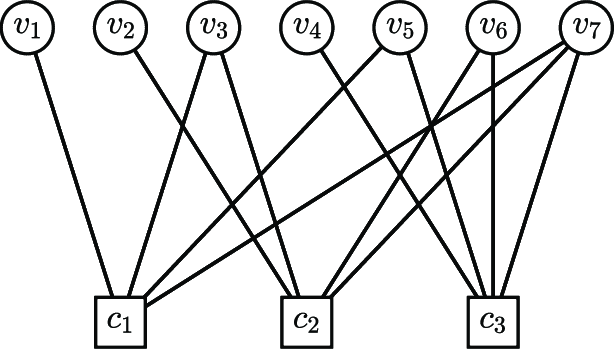
\includegraphics[scale=0.5]{Tanner1.png}  
  \caption{Graphe de Tanner associé}
  \label{fig:Tanner1}
\end{figure}
\clearpage
\textbf{Autre exemple:}
Soit la matrice de Parité : \newline
$$H=
\begin{pmatrix}
  1 & 0 & 0 & 0 & 1 & 0 & 0 & 0 \\
  0 & 1 & 0 & 0 & 1 & 1 & 0 & 0 \\
  
  0 & 0 & 1 & 0 & 0 & 1 & 1 & 0 \\
  0 & 0 & 0 & 1 & 0 & 0 & 1 & 1 
  
  
\end{pmatrix}
\quad
$$
\begin{figure}[!h]
  \centering
  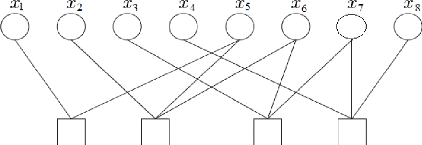
\includegraphics[scale=0.5]{Tanner2.png}  
  \caption{Graphe biparti de Tanner associé}
  \label{fig:Tanner2}
\end{figure}

Le graphe de Tanner est utilisé comme support pour la plupart des algorithmes de décodage. Le principe principal d'un algorithme de décodage utilisant cette 
représentation est de considérer chaque branche du graphe comme un message d'un noeud $c_j$ vers un noeud $v_i$ et réciproquement.

%\subsection{Vocabulaire}
\newpage
%-----------------------------------------------------
%-----------------------------------------------------

\section{Algorithme de décodage}
\label{sec:algo}
Il existe plusieurs types d'algorithmes de décodage pour les codes LDPC. Cependant, nous en avons étudier un seul.
Ce dernier consiste à faire baisser le poids du syndrome jusqu'à que ce dernier soit nul. L'objectif de cet algorithme 
est de relever les colonnes d'une matrice de parité $H$ qui sont erronés.
Pour ce faire, les positions qui sont en erreurs vont faire baisser le poids de notre syndrome. Ainsi, on va parcourir 
chaque colonnes de la matrice $H$ afin de trouver ces dernières.
On définit le code LDPC $C$ à l'aide d'une matrice de parité \textbf{H}, qui est creuse.
Soit $y = x + e$, où $y$ est le message reçu, $x$ le message chiffré et $e$ le vecteur erreur.\vspace{0.4cm}\newline

Voici l'algorithme:\vspace{0.4cm}\newline

\begin{algorithm}[H]
  \SetAlgoLined
  \KwData{Soient $E$ un motif d'erreur et $H$ une matrice de parité de taille $n$. }
  \KwResult{Syndrome de l'erreur courant}

  On définit les $h_{i}$, $\forall i \in \llbracket 0~;~ n \rrbracket$ les colonnes de la matrice H.
  
  Et on note $\omega(e)$ le poids de $e$.

  $S = \sigma(E) = H.~^tE$
  
  %$compteur \leftarrow 0$

  \For{$i\leftarrow 0$ \KwTo $n$}{
     \If{$\omega(S + h_{i}) \le \omega(S)$}{
      $E_1 \leftarrow E_1 + h_i$ 
    }
  }
  \eIf{$S = \omega(E_1)$}{
    le syndrome de l'erreur trouvé est le syndrome de l'erreur courante\;
    \KwRet{$E_1$}
  }{
    on répète l'algorithme avec le nouveau motif d'erreur trouvé\;
    $S = \sigma(E) + \sigma(E_1) = \sigma(E + E_1)$\;
    \KwRet{$E_1 + $} \Repeat{$\omega(S) = 0$}{}
  }
  \caption{Algorithme de décodage LDPC}
\end{algorithm}
\vspace{0.4cm}
On peut remarquer que l'algorithme peut vite faire une boucle infini si la condition à la ligne 
\textbf{\textsc{17}} n'est pas satisfaite.
Nous allons définir un nombre maximal d'itération à exécuter. En effet, il se peut que l'algorithme 
de décodage LDPC ne trouve pas de solution, de ce faite, on évite une boucle infini.\vspace{0.4cm}\newline
Dans notre implémentation Python, nous avons fait le choix d'éxécuter au plus 25 fois la recherche puisque 
si le poids ne diminue plus, on ne peut pas décoder le code LDPC. Nous verrons cela dans la partie \ref{sec:exp}.
\clearpage
\lstinputlisting[language=python, firstline=7, lastline=41]{main.py}
\vspace{0.5cm} Les fonctions auxiliaires apparaissent sur l'annexe \ref{sec:annexe}.
%Pour écrire des algorithmes, le paquetage suivant est très utile : \url{http://tug.ctan.org/macros/latex/contrib/algorithm2e/doc/algorithm2e.pdf}  
\clearpage
%-----------------------------------------------------
%-----------------------------------------------------

\section{Expérimentations et résultats}
\label{sec:exp}

Nous avons réaliser plusieurs types d'expériences. Nous avons découvert que plus la taille des matrices est grande, 
plus l'algorithme de décodage fonctionne. En effet, Pour livrer nos résultats, nous avons choisit des matrices de longueur 
$1000$ et $2000$.

Nous avons implémenter des fonctions\ref{sec:annexe} de façon à pouvoir créer des matrices creuses.
La fonction \textit{matrixFromWeight(poids,n)} créer une matrice de dimension $\dfrac{n}{2}$ par $n$ de tel sorte que 
chaque colonne est un poids de valeur $poids$ et est unique. Sinon, notre matrice de parité ne représente pas un code LDPC régulier.\vspace{0.4cm}\newline
\underline{Objectif de l'expérimentation:} Nous allons essayer de déterminer le poids optimale sur chaque colonne pour décoder un code 
LDPC de longueur $n$.\vspace{0.4cm}\newline
La méthode adopter est la suivante:
\begin{enumerate}
  \item[1.] Construire une matrice dont les colonnes ont un certain poids.
  \item[2.] Observer combien de vecteurs erreurs d'un certain poids, nous arrivons à retrouver grâce à notre algorithme de décodage classique.
  \item[3.] Essayer d'optimiser l'algorithme de décodage en supprimant les position parasites et donc essayer de décoder plus de vecteurs erreurs (ou non).
  \item[4.] Comparer les résultats des deux algorithmes.
\end{enumerate}

\textsc{\textbf{\underline{Remarque :}}} Une position parasite est une colonne de H qui satisfait la condition\newline $\omega(S + h_{i}) \le \omega(S)(1)$ mais qui n'est pas une 
position érronée. En outre, on va durcir la condition $(1)$ de façon a ignorer ces positions. Pour cela, on essaiera de récupérer les colonnes de H qui font baisser le
syndrome. ($\omega(S + h_{i}) < \omega(S)$ ou encore $\omega(S + h_{i}) < \omega(S) - 1$, par exemple)

\subsection{$n = 1000$}
Nous réalisons une série d'expériences sur des matrices de dimension 500 par 1000. Pour ce faire, on regarder combien de vecteurs erreurs
sommes-nous capable de décoder. On se définit un échantillions de 200 vecteurs erreurs puis on calcul la probabilité de décodage en fonction d'un type de matrice donnée.
En effet, on définit une matrice avec un certain poids sur chaque colonne puis on appelle l'algorithme de décodage.\vspace{0.4cm}\newline

La Table \ref{table:res1} présente un résumé des résultats de nos expérimentations pour $n=1000$ à l'aide de la fonction
\textit{decode\_LDPC} (étape 2 de la démarche expérimental). 

La Table \ref{table:res2} présente un résumé des résultats de nos expérimentations pour $n=1000$ à l'aide de la fonction
\textit{decode\_LDPC\_strict} (étape 3 de la démarche expérimental). 
Pour la fonction \textit{decode\_LDPC\_strict}, nous avons choisit d'essayer de faire baisser le poids du syndrome de 2 à la première itération puis de 1 sur les 
deux suivantes. Ensuite, l'algorithme se déroule sans contrainte sur les 22 autres itérations.

\vspace{0.4cm}
On peut observer plusieurs choses. Premièrement, sur la table \ref{table:res1} on arrive à décoder les 200 vecteurs erreurs de poids 
8 sur une matrice dont les colonnes sont de poids 11. Sur cette même colonne, les vecteurs erreurs de poids 7 ne sont pas tous décoder (99\% de décodage).
On peut expliquer cela à cause de l'aléatoire, en effet, nous générons des vecteurs erreurs aléatoirement et des matrices aléatoirement aussi.
Donc il est possible d'obserser ce type de phénomène puisque les positions des 1 ne vont pas s'intersecter. De ce faite,
le poids du syndrome ne va pas diminuer mais augmenter.\newline
Étant donné que nous décodons le plus de vecteurs dont les colonnes sont de poids 11, ce dernier semble être le poids optimale
pour $n = 1000$. Lorqu'on observe la table \ref{table:res2} les résultats sont convainquants jusqu'à des poids 6 sur les vecteurs erreurs.
Mais l'optimale semble se situé entre des poids de colonnes qui se situent entre 10 et 12 inclus. On ne décode pas autant de vecteurs erreurs
car en 25 itérations, nous ne parvenons pas à trouver toutes les solutions.
\clearpage
\underline{Deux explications possible :}
\begin{enumerate}
  \item On diminue trop le poids du syndrome et on oublie des positions
  \item Ou, on exécute pas assez d'itération
\end{enumerate}

Il est difficile de répondre directement à la première explication, cependant on peut lancer nos tests sur plus d'itérations par exemples.
Nous faisons 50. On arrive à observer des résultats similaires que pour 25 itérations. On ne manipule jamais les mêmes matrices ni les même échantillions de vecteurs erreurs
puisque nous générons tout aléatoirement. Parfois, on arrive à décoder les 200 vecteurs erreurs de poids 7 mais le plus souvent non.
On peut donc en déduire expérimentalement que l'on diminue trop le poids du syndrome.\vspace{0.4cm}\newline

\underline{Observations supplémentaire:} L'algortime strict nous permet de décoder beacoup plus de vecteurs erreurs que le premier algorithme. On a fait le choit d'arrêter nos algorithmes
lorque la dernière probabilité de déocdage calculé est inférieur ou égal à 0.8. En effet, nous avons pue observer que dans tous les cas, si on la probabilité chute drastiquement
après ce palier donc nous avons juger ces résulats non pertinent. Donc on peut observer que sur la table \ref{table:res1} les résultats chute d'un coups après que la probabilité de décodage soit 
résonnable. On peut observer ce phénomène sur la colonne des poids 14 par exemple. Si on observe cette même colonne dans la \ref{table:res2} on peut voir que les résultats sont plus lisses.

\subsection{$n = 2000$}
La Table \ref{table:res3} présente un résumé des résultats de nos expérimentations pour $n=2000$ à l'aide de la fonction
\textit{decode\_LDPC\_strict}.\vspace{0.4cm}\newline
Les expériences sur les matrices de dimension $1000$ par $2000$ sont gourmandes en temps et en ressource. La création de la matrice n'est pas instantanée. Par exemple, créer une matrice ayant un poids de 9 sur les colonnes, environ 15 secondes sont nécessaires. 
Ainsi, nous allons présenter 
les résultats de \textit{decode\_LDPC\_strict} sur un échantillions de 25 vecteurs erreurs. Et sur 25 itérations maximale de décodage.\vspace{0.4cm}\newline

On observe que l'algorithme de décodage fonctionne bien, encore mieux que lorsque $n=1000$. On arrive à décoder jusqu'à 25 vecteurs erreurs de poids 21. Ici, encore, on observe le même phénomène qui est 
dû à l'aléatoire. Pour ce poids de colonne, on n'observe pas que des probabilités certaines jusqu'au poids 21, cependant il porte à croire que 9 est le poids optimale pour 
$n = 2000$. En effet, c'est le poids de colonne qui permet de décoder le plus de vecteurs erreurs d'un poids élévé.\vspace{0.4cm}\newline

Dans l'ensemble, on a observé que supprimer les position parasites était beaucoup plus éfficasse pour $n=2000$. En effet, on arrive à gagner en terme de capacité de décodage.
En laissant tourner la fonction sur 50 itérations, on ne parvient pas à obtenir une variations des résultats. On peut observer une amélioration dans la qualité de ces derniers puiqu'on obtient
une série de probabilité qui vaut 1 jusqu'au poids de vecteurs erreur 18.


\clearpage
%-----------------------------------------------------
%-----------------------------------------------------


%% Les appendices commencent après la commande \appendix
%% Les commandes \chapter (si l'option chapter est sélectionnée), \section, \subsection peuvent s'utiliser comme habituellement
%\appendix

%\clearpage % à utiliser pour afficher la biblographie sur une nouvelle page
% References

%\printbibliography
\section{Annexe}
\begin{table}[htbp]
  \centering
  \caption{Probabilité de décodage sur 200 vecteurs erreurs d'un certain poids en fonction du poids des colonnes d'une matrice de code LDPC}
  \label{table:res1}
  \vspace{0.3cm}\hspace{4.5cm} Poids des colonnes\vspace{0.1cm}
  \begin{tabular}{|c|c|c|c|c|c|c|c|c|c|}
    \hline
    Poids des vecteurs erreurs &3 &4 &5 &6 &7 &8 &9 &10 &11 \\
    \hline
    1	&0.915	&0.745	&1.0	&0.96	&0.99	&1.0	&1.0	&1.0	&1.0 \\
    \hline
    2	&-	&-	&1.0	&-	&-	&1.0	&1.0	&1.0	&1.0 \\
    \hline
    3	&-	&-	&1.0	&-	&-	&1.0	&1.0	&1.0	&1.0 \\
    \hline
    4	&-	&-	&1.0	&-	&-	&1.0	&1.0	&1.0	&1.0 \\
    \hline
    5	&-	&-	&1.0	&-	&-	&1.0	&1.0	&1.0	&1.0 \\
    \hline
    6	&-	&-	&0.995	&-	&-	&1.0	&1.0	&1.0	&1.0 \\
    \hline
    7	&-	&-	&1.0	&-	&-	&0.945	&1.0	&0.995	&0.99\\
    \hline
    8	&-	&-	&0.98	&-	&-	&0.74	&0.995	&0.825	&1.0 \\
    \hline
    9	&-	&-	&0.975	&-	&-	&-	&0.985	&0.55	&0.98 \\
    \hline
    10	&-	&-	&0.95	&-	&-	&-	&0.955	&-	&0.915 \\
    \hline
    11 	&-	&-	&0.925	&-	&-	&-	&0.885	&-	&0.725 \\
    \hline
    12	&-	&-	&0.87	&-	&-	&-	&0.75	&-	&- \\
    \hline
    13	&-	&-	&0.775	&-	&-	&-	&-	&-	&- \\
    \hline
    Temps CPU (s) &263	&560	&3458	&203	&131	&3050	&3318	&3176	&2748\\
    \hline
    - &- &- &- &- &- &- &- &- &-\\
    \hline
    Poids des vecteurs erreurs &\phantom &12 &13 &14 &15 &16 &17 &18 &19 \\
    \hline
    1 &\phantom &1.0	&1.0	&1.0	&1.0	&1.0	&1.0	&1.0	&1.0 \\
    \hline
    2 &\phantom&1.0	&1.0	&1.0 &1.0	&1.0	&1.0	&1.0	&1.0\\
    \hline
    3 &\phantom &1.0	&1.0	&1.0	&1.0	&1.0	&1.0	&1.0	&1.0 \\
    \hline
    4 &\phantom &1.0	&1.0	&1.0	&1.0	&1.0	&1.0	&1.0	&1.0 \\
    \hline
    5 &\phantom &1.0	&1.0	&1.0	&0.995	&1.0	&0.995	&0.995	 &0.985 \\
    \hline
    6 &\phantom &1.0	&1.0	&1.0	&1.0	&1.0	&0.985	&0.985	&1.0 \\
    \hline
    7 &\phantom &0.985	&1.0	&0.99	&0.995	&0.955	&0.97	&0.92	&0.995 \\
    \hline
    8 &\phantom &0.905	&0.985	&0.8	&0.99	&0.685	&0.955	&0.605	&0.93 \\
    \hline
    9 &\phantom &0.51	&0.97	&0.395	&0.94	&-	&0.895	&-	&0.645 \\
    \hline
    10 &\phantom &-	&0.855	&-	&0.76	&-	&0.8	&-	&- \\
    \hline
    11 &\phantom  &-	&0.57	&-	&-	&-	&0.58	&-	&- \\
    \hline
    12 &\phantom &-	&-	&-	&-	&-	&-	&-	&- \\
    \hline
    13 &\phantom &-	&-	&-	&-	&-	&-	&-	&- \\
    \hline
    Temps CPU (s) &\phantom &4246	&5099	&4169	&2204	&1968	&4503	&2317	&1997\\
    \hline
  \end{tabular}
\end{table}%
\clearpage
\begin{table}[htbp]
  \centering
  \caption{Probabilité de décodage sur 200 vecteurs erreurs d'un certain poids en fonction du poids des colonnes d'une matrice de code LDPC}
  \vspace{0.3cm}\hspace{4.5cm} Poids des colonnes\vspace{0.1cm}
  \label{table:res2}
  \begin{tabular}{|c|c|c|c|c|c|c|c|c|c|}
          \hline
          Poids des vecteurs erreurs &3 &4 &5 &6 &7 &8 &9 &10 &11 \\
          \hline
          1 &1.0	&1.0	&1.0 &1.0	&1.0 &1.0	&1.0 &1.0 &1.0 \\
          \hline
          2 &1.0	&1.0	&1.0 &1.0	&1.0 &1.0	&1.0 &1.0 &1.0 \\
          \hline
          3 &0.97	&1.0 &0.99 &1.0 &1.0 &1.0 &0.995 &1.0 &1.0 \\
          \hline
          4 &0.895 &0.99 &0.99 &0.99 &1.0 &1.0 &1.0 &1.0 &0.99 \\
          \hline
          5	&0.835 &0.98 &0.965 &0.995 &0.99 &0.995 &0.99 &1.0 &0.99 \\
          \hline
          6	&0.725 &0.97 &0.91 &0.975 &0.95 &0.985 &0.985 &1.0 &0.99 \\
          \hline
          7	&- &0.945 &0.82 &0.96 &0.915 &0.98 &0.96 &0.975 &0.965 \\
          \hline
          8	&- &0.905 &0.81 &0.965 &0.865 &0.965 &0.925 &0.97 &0.915 \\
          \hline
          9	&- &0.86 &0.67 &0.905 &0.835 &0.925 &0.91 &0.955 &0.88 \\
          \hline
          10 &- &0.82 &- &0.885 &0.825 &0.9	&0.81	&0.93	&0.81 \\
          \hline
          11 &- &0.775 &-	&0.845 &0.635	&0.845 &0.705	&0.855 &0.725 \\
          \hline
          12 &- &- &- &0.785	&- &0.825 &- &0.82 &- \\
          \hline
          13 &- &- &- &- &- &0.69 &- &0.745	&- \\
          \hline
          Temps CPU (s) &890 &2082 &1405 &2035 &1475 &3694 &1457 &1953 &1661\\
          \hline
          - &- &- &- &- &- &- &- &- &-\\
          \hline
          Poids des vecteurs erreurs &\phantom &12 &13 &14 &15 &16 &17 &18 &19 \\
          \hline
          1 &\phantom &1.0	&1.0	&1.0	&1.0	&1.0	&1.0	&1.0	&1.0 \\
          \hline
          2 &\phantom&1.0	&1.0	&1.0 &1.0	&1.0	&1.0	&1.0	&1.0\\
          \hline
          3 &\phantom &1.0	&1.0	&1.0	&1.0	&1.0	&1.0	&1.0	&1.0 \\
          \hline
          4 &\phantom &1.0	&1.0	&1.0	&1.0	&1.0	&1.0	&1.0	&1.0 \\
          \hline
          5 &\phantom &0.995	&0.995	&1.0	&1.0	&1.0	&0.995	&1.0	 &0.995 \\
          \hline
          6 &\phantom &1.0	&0.985 &1.0	&0.99	&0.995	&0.985	&0.995	&0.985 \\
          \hline
          7 &\phantom &0.995	&0.96	&0.99	&0.98	&0.99	&0.97	&0.98	&0.975 \\
          \hline
          8 &\phantom &0.985	&0.93	&0.98	&0.94	&0.945	&0.955	&0.95	&0.935 \\
          \hline
          9 &\phantom &0.95	&0.9	&0.965	&0.865	&0.9	&0.895	&0.935	&0.81 \\
          \hline
          10 &\phantom  &0.905	&0.83	&0.935	&0.78	&0.83	&0.8	&0.785	&0.7 \\
          \hline
          11 &\phantom  &0.85	&0.745	&0.855	&-	&0.655	&0.58	&-	&- \\
          \hline
          12 &\phantom &0.82	&-	&0.7	&-	&-	&-	&-	&- \\
          \hline
          13 &\phantom &0.625	&-	&-	&-	&-	&-	&-	&- \\
          \hline
          Temps CPU (s) &\phantom &2652 &1629	&3899 &1297	&1951	&1456	&1609	&1606\\
          \hline
  \end{tabular}
\end{table}%

\begin{table}[htbp]
  \centering
  \caption{Probabilité de décodage sur 25 vecteurs erreurs d'un certain poids en fonction du poids des colonnes d'une matrice de code LDPC (n=2000)}
  \label{table:res3}
  \vspace{0.1cm}\hspace{4.5cm} Poids des colonnes\vspace{0.1cm}
  \begin{tabular}{|c|c|c|c|c|c|c|c|c|c|c|}
    \hline
    Poids des vecteurs erreurs &3 &4 &5 &6 &7 &8 &9 &10 &11 &12\\
    \hline
    1	&1.0	&1.0	&1.0	&1.0	&1.0	&1.0	&1.0	&1.0	&1.0 &1.0\\
    \hline
    2	&1.0	&1.0	&1.0	&1.0	&1.0	&1.0	&1.0	&1.0	&1.0 &1.0\\
    \hline
    3	&1.0	&1.0	&1.0	&1.0	&1.0	&1.0	&1.0	&1.0	&1.0 &1.0\\
    \hline
    4	&0.92	&1.0	&1.0	&1.0	&1.0	&1.0	&1.0	&1.0	&1.0 &1.0\\
    \hline
    5	&0.88	&1.0	&1.0	&1.0	&1.0	&1.0	&1.0	&1.0	&1.0 &1.0\\
    \hline
    6	&0.76	&1.0	&1.0	&1.0	&1.0	&1.0	&1.0	&1.0	&1.0 &1.0 \\
    \hline
    7	&-	&0.96	&1.0	&1.0	&1.0	&1.0	&1.0	&1.0	&1.0	&1.0 \\
    \hline
    8	&-	&1.0	&1.0	&1.0	&1.0	&1.0	&1.0	&1.0	&1.0	&1.0 \\
    \hline
    9	&-	&0.92	&1.0	&1.0	&1.0	&1.0	&1.0	&1.0	&0.96	&1.0 \\
    \hline
    10	&-	&1.0	&0.92	&0.96	&0.92	&0.96	&1.0	&1.0	&0.96	&0.96 \\
    \hline
    11	&-	&0.96	&0.88	&1.0	&0.96	&1.0	&1.0	&1.0	&1.0	&0.96 \\
    \hline
    12	&-	&0.8	&0.88	&0.96	&0.92	&0.96	&0.96	&1.0	&1.0	&1.0 \\
    \hline
    13	&-	&0.88	&0.76	&0.92	&0.92	&1.0	&1.0	&1.0	&0.92	&1.0 \\
    \hline
    14	&-	&0.72	&-	&0.88	&0.8	&0.92	&1.0	&0.96	&0.88	&1.0 \\
    \hline
    15	&-	&-	&-	&1.0	&0.76	&1.0	&0.92	&0.96	&0.8	&0.96 \\
    \hline 
    16	&-	&-	&-	&0.84	&-	&1.0	&1.0	&0.84	&0.92	&1.0 \\
    \hline
    17	&-	&-	&-	&0.76	&-	&0.96	&0.92	&0.88	&0.96	&0.88 \\
    \hline 
    18	&-	&-	&-	&-	&-	&0.92	&1.0	&0.88	&0.84	&0.84 \\
    \hline
    19	&-	&-	&-	&-	&-	&0.84	&0.96	&0.84	&0.8	&0.8 \\
    \hline
    20	&-	&-	&-	&-	&-	&0.92	&0.84	&0.76	&0.76	&0.88 \\
    \hline
    21	&-	&-	&-	&-	&-	&0.72	&1.0	&-	&-	&0.8 \\
    \hline
    22	&-	&-	&-	&-	&-	&-	&0.88	&-	&-	&0.72 \\
    \hline
    23	&-	&-	&-	&-	&-	&-	&0.8	&-	&-	&- \\
    \hline
    24	&-	&-	&-	&-	&-	&-	&0.72	&-	&-	&- \\
    \hline
    - &- &- &- &- &- &- &- &- &-\\
    \hline
    Poids des vecteurs erreurs &13 &14 &15 &16 &17 &18 &19 &20 &21 &22\\
    \hline
    1 &1.0	&1.0	&1.0	&1.0	&1.0	&1.0	&1.0	&1.0	&1.0	&1.0 \\
    \hline
    2 &1.0	&1.0	&1.0	&1.0	&1.0	&1.0	&1.0	&1.0	&1.0	&1.0 \\
    \hline
    3 &1.0	&1.0	&1.0	&1.0	&1.0	&1.0	&1.0	&1.0	&1.0	&1.0 \\
    \hline
    4 &1.0	&1.0	&1.0	&1.0	&1.0	&1.0	&1.0	&1.0	&1.0	&1.0 \\
    \hline
    5 &1.0	&1.0	&1.0	&1.0	&1.0	&1.0	&1.0	&1.0	&1.0	&1.0 \\
    \hline
    6 &1.0	&1.0	&1.0	&1.0	&1.0	&1.0	&1.0	&1.0	&1.0	&1.0 \\
    \hline
    7 &1.0	&1.0	&1.0	&1.0	&1.0	&1.0	&1.0	&1.0	&1.0	&1.0 \\
    \hline
    8&1.0	&1.0	&1.0	&1.0	&1.0	&1.0	&1.0	&1.0	&1.0	&1.0 \\
    \hline
    9&1.0	&1.0	&1.0	&1.0	&1.0	&1.0	&1.0	&1.0	&1.0	&1.0 \\
    \hline
    10&1.0	&1.0	&1.0	&1.0	&1.0	&1.0	&1.0	&1.0	&1.0	&1.0 \\
    \hline
    11&1.0	&1.0	&1.0	&0.96	&1.0	&0.96	&1.0	&1.0	&1.0	&1.0 \\
    \hline
    12&1.0	&1.0	&0.96	&1.0	&1.0	&0.96	&1.0	&0.96	&1.0	&1.0 \\
    \hline
    13&1.0	&1.0	&1.0	&1.0	&1.0	&0.92	&0.96	&1.0	&1.0	&0.88 \\
    \hline
    14&1.0	&0.96	&0.96	&1.0	&1.0	&1.0	&1.0	&0.92	&0.96	&1.0 \\
    \hline
    15&0.96	&0.92	&1.0	&0.96	&1.0	&0.92	&1.0	&0.92	&0.96	&0.84 \\
    \hline
    16&1.0	&0.88	&1.0	&0.92	&1.0	&0.96	&0.96	&0.7	&0.84	&0.92 \\
    \hline
    17&1.0	&0.84	&1.0	&0.88	&0.84	&0.96	&0.96	&-	&0.56	&0.92 \\
    \hline
    18&0.96	&0.8	&0.84	&0.84	&0.88	&0.76	&0.48	&-	&-	&0.68 \\
    \hline
    19&0.88	&0.92	&0.88	&0.8	&0.64	&-	&-	&-	&-	&- \\
    \hline
    20&0.7	&0.88	&0.72	&0.84	&-	&-	&-	&-	&-	&- \\
    \hline
    21&-	&0.64	&-	&0.48	&-	&-	&-	&-	&-	&- \\
    \hline
    22&-	&-	&-	&-	&-	&-	&-	&-	&-	&- \\
    \hline
    23&-	&-	&-	&-	&-	&-	&-	&-	&-	&- \\
    \hline
    24&-	&-	&-	&-	&-	&-	&-	&-	&-	&- \\
    \hline
  \end{tabular}
\end{table}%
\clearpage
\section{Implémentation}
\label{sec:annexe}
\underline{Fichier tools.py}
\lstinputlisting[language=python]{tools.py}
\mbox{}\hfill\rule{0.5\linewidth}{1mm}\hfill\mbox{}
\vspace{0.3cm}\newline
\underline{Fichier matrix.py}
\lstinputlisting[language=python]{matrix.py}
\mbox{}\hfill\rule{0.5\linewidth}{1mm}\hfill\mbox{}
\vspace{0.3cm}\newline
\underline{Fichier main.py}
\lstinputlisting[language=python]{main.py}


\end{document}
